\documentclass[12pt]{article}

\usepackage{amsmath,amssymb,amsthm}
\usepackage{graphicx}
\usepackage[margin=1in]{geometry}

\begin{document}

\title{\textbf{Hedging Strategies with Perpetuals for Uniswap V4 Liquidity Positions}}
\author{%
  \textbf{Xtreamly}%
}
\date{\today}
\maketitle

\begin{abstract}
This document examines the use of perpetual futures to hedge Uniswap V4 concentrated liquidity positions. By combining long and short perpetual strategies, liquidity providers can reduce downside risk and participate in further price appreciation. The impact of leverage, funding costs, and liquidation risks is discussed, highlighting the importance of optimization and backtesting for effective risk management.
\end{abstract}

\section{Value of a Uniswap V4 Position (Ignoring Fees)}
\label{sec:uniswaplp}

Consider a Uniswap V4 position providing liquidity between the lower price bound and upper bound. For concreteness, suppose we are providing liquidity in the ETH/USDT pool:
\begin{itemize}
    \item \textbf{ETH (token0)} is the volatile asset.
    \item \textbf{USDT (token1)} is the stable asset (or stable-ish).
\end{itemize}

\subsection{Notation}
We define the following variables:
\begin{itemize}
    \item $P_L$: The lower bound price of the LP position (USDT per ETH).
    \item $P_U$: The upper bound price of the LP position (USDT per ETH).
    \item $P$: The current market price of ETH in USDT.
    \item $L$: The \emph{constant} liquidity associated with the position.
    \item $X_0$: The amount of ETH (token0) held at the time the position is set, related to $P_U$ and $P_L$.
    \item $Y_0$: The amount of USDT (token1) held at the time the position is set, also related to $P_U$ and $P_L$.
\end{itemize}

\begin{center}
\textbf{Ignoring fees}, the LP payoff depends on which region the price $P$ falls into:
\end{center}

\subsection{Three Cases for the LP Value}

\textbf{Case 1: Within Range} $P_L \le P \le P_U$ 

\medskip

When the market price $P$ lies within the liquidity provider's chosen range $[P_L, P_U]$, the position consists of a mix of ETH and USDT. The exact amounts of each asset are determined by Uniswap's liquidity formula.

\medskip

At any price $P$ in this range:
\[
X(P) = L \biggl(\frac{1}{\sqrt{P}} - \frac{1}{\sqrt{P_U}}\biggr),
\qquad
Y(P) = L \bigl(\sqrt{P} - \sqrt{P_L}\bigr).
\]
where:
\begin{itemize}
    \item $X(P)$ represents the amount of ETH (token0) held at price $P$.
    \item $Y(P)$ represents the amount of USDT (token1) held at price $P$.
    \item $L$ is the total liquidity provided to the range.
\end{itemize}

The total value of the LP position at price $P$ is then:
\[
V(P) = X(P) \cdot P \;+\; Y(P).
\]

Expanding:
\[
V(P) = L \biggl(\frac{1}{\sqrt{P}} - \frac{1}{\sqrt{P_U}}\biggr) P
\;+\;
L \bigl(\sqrt{P} - \sqrt{P_L}\bigr),
\quad \text{for } P_L \le P \le P_U.
\]

\medskip

\textbf{Case 2: Below Range} $P < P_L$.

\medskip

When the price drops below $P_L$, the liquidity position has been fully converted into ETH (token0). This happens because as price decreases, the Uniswap AMM mechanism sells all available USDT in exchange for ETH.

\medskip

The ETH amount is locked at the value it had at $P_L$, which is:
\[
X(P_L) = L \biggl(\frac{1}{\sqrt{P_L}} - \frac{1}{\sqrt{P_U}}\biggr).
\]
Since the LP now holds only ETH, the total position value in USD is simply the ETH amount multiplied by the current price $P$:
\[
V(P) = X(P_L) \cdot P.
\]
Expanding:
\[
V(P) = L \biggl(\frac{1}{\sqrt{P_L}} - \frac{1}{\sqrt{P_U}}\biggr) P,
\quad \text{for } P < P_L.
\]

\medskip

\textbf{Case 3: Above Range} $P > P_U$.

\medskip

When the price moves above $P_U$, the liquidity position has been fully converted into USDT (token1). This happens because as price increases, the Uniswap AMM mechanism sells all available ETH in exchange for USDT.

\medskip

The USDT amount is locked at the value it had at $P_U$, which is:
\[
Y(P_U) = L \bigl(\sqrt{P_U} - \sqrt{P_L}\bigr).
\]
Since the LP now holds only USDT, the total position value remains constant:
\[
V(P) = Y(P_U).
\]
Expanding:
\[
V(P) = L \bigl(\sqrt{P_U} - \sqrt{P_L}\bigr),
\quad \text{for } P > P_U.
\]

\medskip

\paragraph{Final Piecewise Formula.}
Bringing everything together, the complete value function for the LP position is:
\[
V(P) =
\begin{cases}
L \biggl(\frac{1}{\sqrt{P_L}} - \frac{1}{\sqrt{P_U}}\biggr) P, & P < P_L,\\[8pt]
L \Bigl(\bigl(\tfrac{1}{\sqrt{P}} - \tfrac{1}{\sqrt{P_U}}\bigr) P + \bigl(\sqrt{P} - \sqrt{P_L}\bigr)\Bigr), & P_L \le P \le P_U,\\[10pt]
L \bigl(\sqrt{P_U} - \sqrt{P_L}\bigr), & P > P_U.
\end{cases}
\]

\begin{figure}[htb]
    \centering
    \includegraphics[width=0.7\textwidth]{images/CLposition.png}
    \caption{illustrating the piecewise value of a Uniswap V4 position (ignoring fees).}
    \label{fig:CLposition}
\end{figure}

\newpage

\section{Introducing a Perpetual Hedge}
\label{sec:perphedge}

We consider a perpetual futures contract to hedge ETH/USDT. Let:
\begin{itemize}
    \item $M$: The margin (in USDT) posted for the perpetual position.
    \item $\alpha$: The \emph{notional} size of the perp (in ETH units).
    \item $P_0$: The entry price (USDT per ETH).
    \item $P_{\mathrm{liq}}$: The \emph{liquidation price}, where margin is depleted and lost.\footnote{
      In practice, exchanges might have partial liquidations or maintenance margins, but here we simplify: once $P$ hits $P_{\mathrm{liq}}$, the entire margin $M$ is lost.}
\end{itemize}

\paragraph{Short Perpetual.}  
Suppose we \emph{short} at price $P_0$. The PnL from the short is $\alpha\,(P_0 - P)$. We post margin $M$ to cover losses if $P$ rises. We define $P_{\mathrm{liq}}$ so that when $P = P_{\mathrm{liq}}$, our margin is fully exhausted:
\[
M + \alpha\,(P_0 - P_{\mathrm{liq}}) = 0
\quad\Longrightarrow\quad
P_{\mathrm{liq}} = P_0 + \frac{M}{\alpha}.
\]
Hence, our \textbf{short} payoff is
\[
V_{\mathrm{short}}(P) = 
\begin{cases}
M + \alpha\,(P_0 - P), & P < P_{\mathrm{liq}},\\
-M, & P \ge P_{\mathrm{liq}}.
\end{cases}
\]

\begin{figure}[htb]
    \centering
    \includegraphics[width=0.6\textwidth]{images/short.png}
    \caption{Piecewise payoff for the Short Perpetual, showing the drop to $-M$ at liquidation.}
    \label{fig:short}
\end{figure}

\paragraph{Long Perpetual.}  
If we \emph{long} at $P_0$, the PnL is $\alpha\,(P - P_0)$. The margin $M$ is depleted if $P$ falls by enough. Setting $P = P_{\mathrm{liq}}$ where margin is exhausted:
\[
M + \alpha\,(P_{\mathrm{liq}} - P_0) = 0
\quad\Longrightarrow\quad
P_{\mathrm{liq}} = P_0 - \frac{M}{\alpha}.
\]
Hence, our \textbf{long} payoff is
\[
V_{\mathrm{long}}(P) = 
\begin{cases}
-M, & P \le P_{\mathrm{liq}},\\
\alpha\,(P - P_0), & P > P_{\mathrm{liq}}.
\end{cases}
\]

\begin{figure}[htb]
    \centering
    \includegraphics[width=0.6\textwidth]{images/long.png}
    \caption{Piecewise payoff for the Long Perpetual, showing the drop to $-M$ at liquidation.}
    \label{fig:long}
\end{figure}

\paragraph{Interpretation.}  
At liquidation ($P = P_{\mathrm{liq}}$), the payoff \emph{jumps} from some positive level (on the linear portion) down to $-M$, reflecting full loss of the margin. This discontinuous drop represents the complete loss of collateral at the liquidation boundary.


\section{Combining LP and Perpetual}
\label{sec:fiveway}

In this section, we analyze the combination of a Uniswap V4 concentrated liquidity (CL) position with a perpetual hedge. The goal is to dynamically hedge the price exposure of the LP position while maintaining capital efficiency. \\

\medskip

\subsection{Long Perpetual Hedge with Concentrated Liquidity}

In Figure~\ref{fig:combined-long}, we illustrate the combined payoff of a long perpetual hedge with a Uniswap CL position. This approach is used when the AI expects volatility and wants to ensure exposure to price appreciation of the underlying asset (ETH in our example). Without a hedge, once the price moves above $P_U$, the LP position fully converts into USDT, leading to missed upside. By incorporating a long perpetual hedge, the strategy ensures that additional gains can be captured.

\medskip

\textbf{Key observations from Figure~\ref{fig:combined-long}:}
\begin{itemize}
    \item The Uniswap CL position alone (dashed gray line) exhibits a flat payoff above $P_U$, since all liquidity has been converted to USDT.
    \item The long perpetual hedge introduces a positive slope above the entry price, capturing further upside.
    \item If the price declines and liquidation occurs, the strategy incurs a sharp loss at $P_{\mathrm{liq}}$.
\end{itemize}

\begin{figure}[htb]
    \centering
    \includegraphics[width=0.6\textwidth]{images/combined_long.png}
    \caption{Example combined payoff: Concentrated liquidity plus a Long Perp.}
    \label{fig:combined-long}
\end{figure}

\subsection{Short Perpetual Hedge with Concentrated Liquidity}

In Figure~\ref{fig:combined-short}, we show the combined payoff of a short perpetual hedge with a Uniswap CL position. This strategy is employed when we seek to protect against downside risk. Without a hedge, if the price drops below $P_L$, the position converts entirely into ETH, exposing the LP to further losses. A short perpetual hedge compensates for these losses.

\medskip

\textbf{Key observations from Figure~\ref{fig:combined-short}:}
\begin{itemize}
    \item The Uniswap CL position alone (dashed gray line) exhibits a linear decline below $P_L$ due to full conversion into ETH.
    \item The short perpetual hedge introduces a slope below the entry price, mitigating further downside.
    \item If the price increases and liquidation occurs, the hedge incurs a sharp loss at $P_{\mathrm{liq}}$.
\end{itemize}

\medskip

\begin{figure}[htb]
    \centering
    \includegraphics[width=0.6\textwidth]{images/combined_short.png}
    \caption{Example combined payoff: Concentrated liquidity plus a Short Perp.}
    \label{fig:combined-both}
\end{figure}

Figure~\ref{fig:combined-both} illustrates the combined payoff when using both a short and long perpetual hedge alongside a Uniswap CL position. This configuration aims to provide protection on both the downside and upside, mitigating the risk of price movements that push the LP position out of range.

\medskip

\textbf{Key insights:}
\begin{itemize}
    \item The long perpetual hedge compensates for missed upside when the price surpasses $P_U$, ensuring the strategy does not forgo further gains once the LP position is fully converted to USDT.
    \item The short perpetual hedge offsets losses when the price declines below $P_L$, counteracting the exposure to ETH that would otherwise be unhedged.
    \item The combined strategy flattens the risks associated with concentrated liquidity by maintaining a more balanced exposure across price ranges.
\end{itemize}

However, this strategy is not without risks. If the price oscillates too frequently around the entry levels of the perpetual positions, liquidations can occur before meaningful profits are realized. This would result in accumulated losses, as the hedges fail to serve their intended purpose of long-term exposure management. 

\medskip

Thus, to maximize the effectiveness of this combined approach, it is crucial to:
\begin{itemize}
    \item Optimize hedge sizing to avoid excessive liquidation risk while maintaining capital efficiency.
    \item Adjust leverage cautiously, as higher leverage increases sensitivity to liquidation but also amplifies returns when successful.
    \item Backtest under different market conditions to analyze whether the perpetual hedges improve overall strategy performance or lead to excessive churn.
\end{itemize}

Overall, the combined approach offers significant downside protection and potential for additional upside capture, but requires careful risk management to prevent liquidation losses from overwhelming the benefits of the hedging strategy.

\subsection{Considerations for Hedge Optimization}

The effectiveness of this strategy depends on proper hedge allocation and leverage management:
\begin{itemize}
    \item \textbf{Collateral allocation:} The fraction of total capital allocated to the hedge determines its impact on the overall payoff.
    \item \textbf{Leverage choice:} Higher leverage increases capital efficiency but also raises funding costs and liquidation risk.
    \item \textbf{Funding rate impact:} Perpetual futures often have non-zero funding rates, which can accumulate over time, affecting profitability.
    \item \textbf{Backtesting necessity:} The interaction between CL payoffs and perpetual hedges needs to be tested across various market conditions to ensure robustness.
\end{itemize}

By systematically balancing these parameters, liquidity providers can dynamically adjust their hedge exposure, optimizing for capital efficiency while managing risk exposure.

\begin{figure}[htb]
    \centering
    \includegraphics[width=0.6\textwidth]{images/combined_both.png}
    \caption{Example combined payoff: Concentrated liquidity plus a Short and Long Perp.}
    \label{fig:combined-short}
\end{figure}

\newpage

\section{Application of Hedging for Historical Positions in Uniswap Pool ETH/USDT}
\label{sec:hedgingmechanism}

We propose an initial hedging methodology by leveraging Uniswap V4's latest hook capabilities to open hedging perpetual positions with mirror funds on the GMX exchange. The goal is to mitigate impermanent loss by stabilizing the payoff function to be market neutral and, when possible, improve market efficiency for Uniswap while enhancing collected fees for the user. The hook mechanism automates the process of splitting initial funding, ensuring seamless integration of the hedging strategy within Uniswap’s smart contract framework.

\subsection{Hedging Mechanism}

\paragraph{Liquidity Provision Setup:} 
We presume entering hedged lp position is the same as in Uniswap v3.
\begin{itemize}
	\item $P_L$: The lower bound price of the LP position (USDT per ETH).
	\item $P_U$: The upper bound price of the LP position (USDT per ETH).
	\item $X_0$: The amount of ETH (token0) held at the time the position is set, related to $P_U$ and $P_L$.
	\item $Y_0$: The amount of USDT (token1) held at the time the position is set, also related to $P_U$ and $P_L$.
\end{itemize}
The total value of deposited tokens is considered the user's original investment.

\paragraph{Triggering the Hedging Mechanism:} 
The hedging mechanism is activated only when Xtreamly AI predicts 'low volatility.' This ensures that hedging is only applied in stable market conditions, reducing the risk of perpetual liquidation due to sudden price swings.

\paragraph{Fund Allocation at Position Opening:} 
We presume entering hedged lp position is the same as in Uniswap v3.
\begin{itemize}
	\item \textbf{80\%} of the funds are allocated to the Uniswap LP position, structured with the same price bounds as the original deposit but proportionally reduced.
	\item \textbf{20\%} is allocated to a hedging perpetual futures position.
\end{itemize}

\paragraph{Perpetual Hedge Positioning:} 

\begin{itemize}
	\item The perpetual hedge is a short position using the allocated 20\% as collateral.
	\item The leverage is determined to ensure that the liquidation price of the perpetual position is slightly above the upper price bound, using the formula:
	$$Leverage_GMX = int(\min(10,\max(1,  \frac{1}{\frac{P_U}{P}-1})))$$
	where $\max 10$ relates to 10\% of the price buffer; and $\min 1$ avoid excessively loose hedging ranges.
\end{itemize}
This approach accounts for the highly volatile nature of Uniswap pools and optimizes the risk-reward balance in the hedging strategy. 

\subsection{Assumptions on GMX Parameters}
The following GMX trading parameters are assumed:
\begin{itemize}
	\item \textbf{Entry fee}: 0.1\%
	\item \textbf{Exit fee}: 0.1\%
	\item \textbf{Gas fee}: Considered negligible due to GMX's efficient execution model.
	\item \textbf{Funding rate}: 0.01\% (assumed constant and charged on an hourly basis).
	\item \textbf{Maximum perpetual duration}: 24 hours. Due to the perpetual funding rate cost, positions cannot be held indefinitely without eroding hedging benefits.	
\end{itemize}

\subsection{Assumptions on Selecting Uniswap Positions for Backtesting}
For backtesting, we identified LP Positions in Uniswap Pool ETH/USDT 0.3\% Fee, that will be used to evaluate the effectiveness of our hedging strategy under different market conditions, comparing LP-only positions against LP positions with perpetual hedging.

\paragraph{Selection Criteria:}
To ensure computational simplicity and practical relevance, we apply the following selection constraints:
\begin{itemize}
	\item \textbf{Period}: LP positions must have been opened and closed between 2024-10-01 and 2024-12-31.
	\item \textbf{Minimum duration}: 60 minutes to avoid Just-In-Time (JIT) positions and ensure sufficient market impact assessment.
	\item \textbf{Concentration levels}: The difference between upper and lower price bounds relative to the deposited price must not exceed 30\%. This aligns with Uniswap V3 \& V4 efficient liquidity allocation principles, ensuring that leveraged hedging is effective.
	\item \textbf{Simplistic positions}: We select only positions consisting of three transaction logs: deposit tokens, withdraw tokens, and collected fees. This simplification facilitates efficient backtesting as a tradeoff of simplicity.
	\item \textbf{No assumptions on position value}: The strategy is applied across a range of liquidity sizes.
\end{itemize}
By applying these filters, we ensure realistic hedging conditions where the strategy remains both practical and effective.

\subsection{Monitoring Performance of Hedged LP Positions}
To evaluate performance, we simulate LP positions and perpetual positions simultaneously by applying the hedging mechanism to historical data.

\paragraph{Sample Position Hedging}
Given the criteria and mechanism described before, here is a sample hedging visualization of position ID \textbf{$840439_0x4942e2b839fc479c27c496b7758bab94ceb6b684$}.
\begin{figure}[htb]
	\centering
	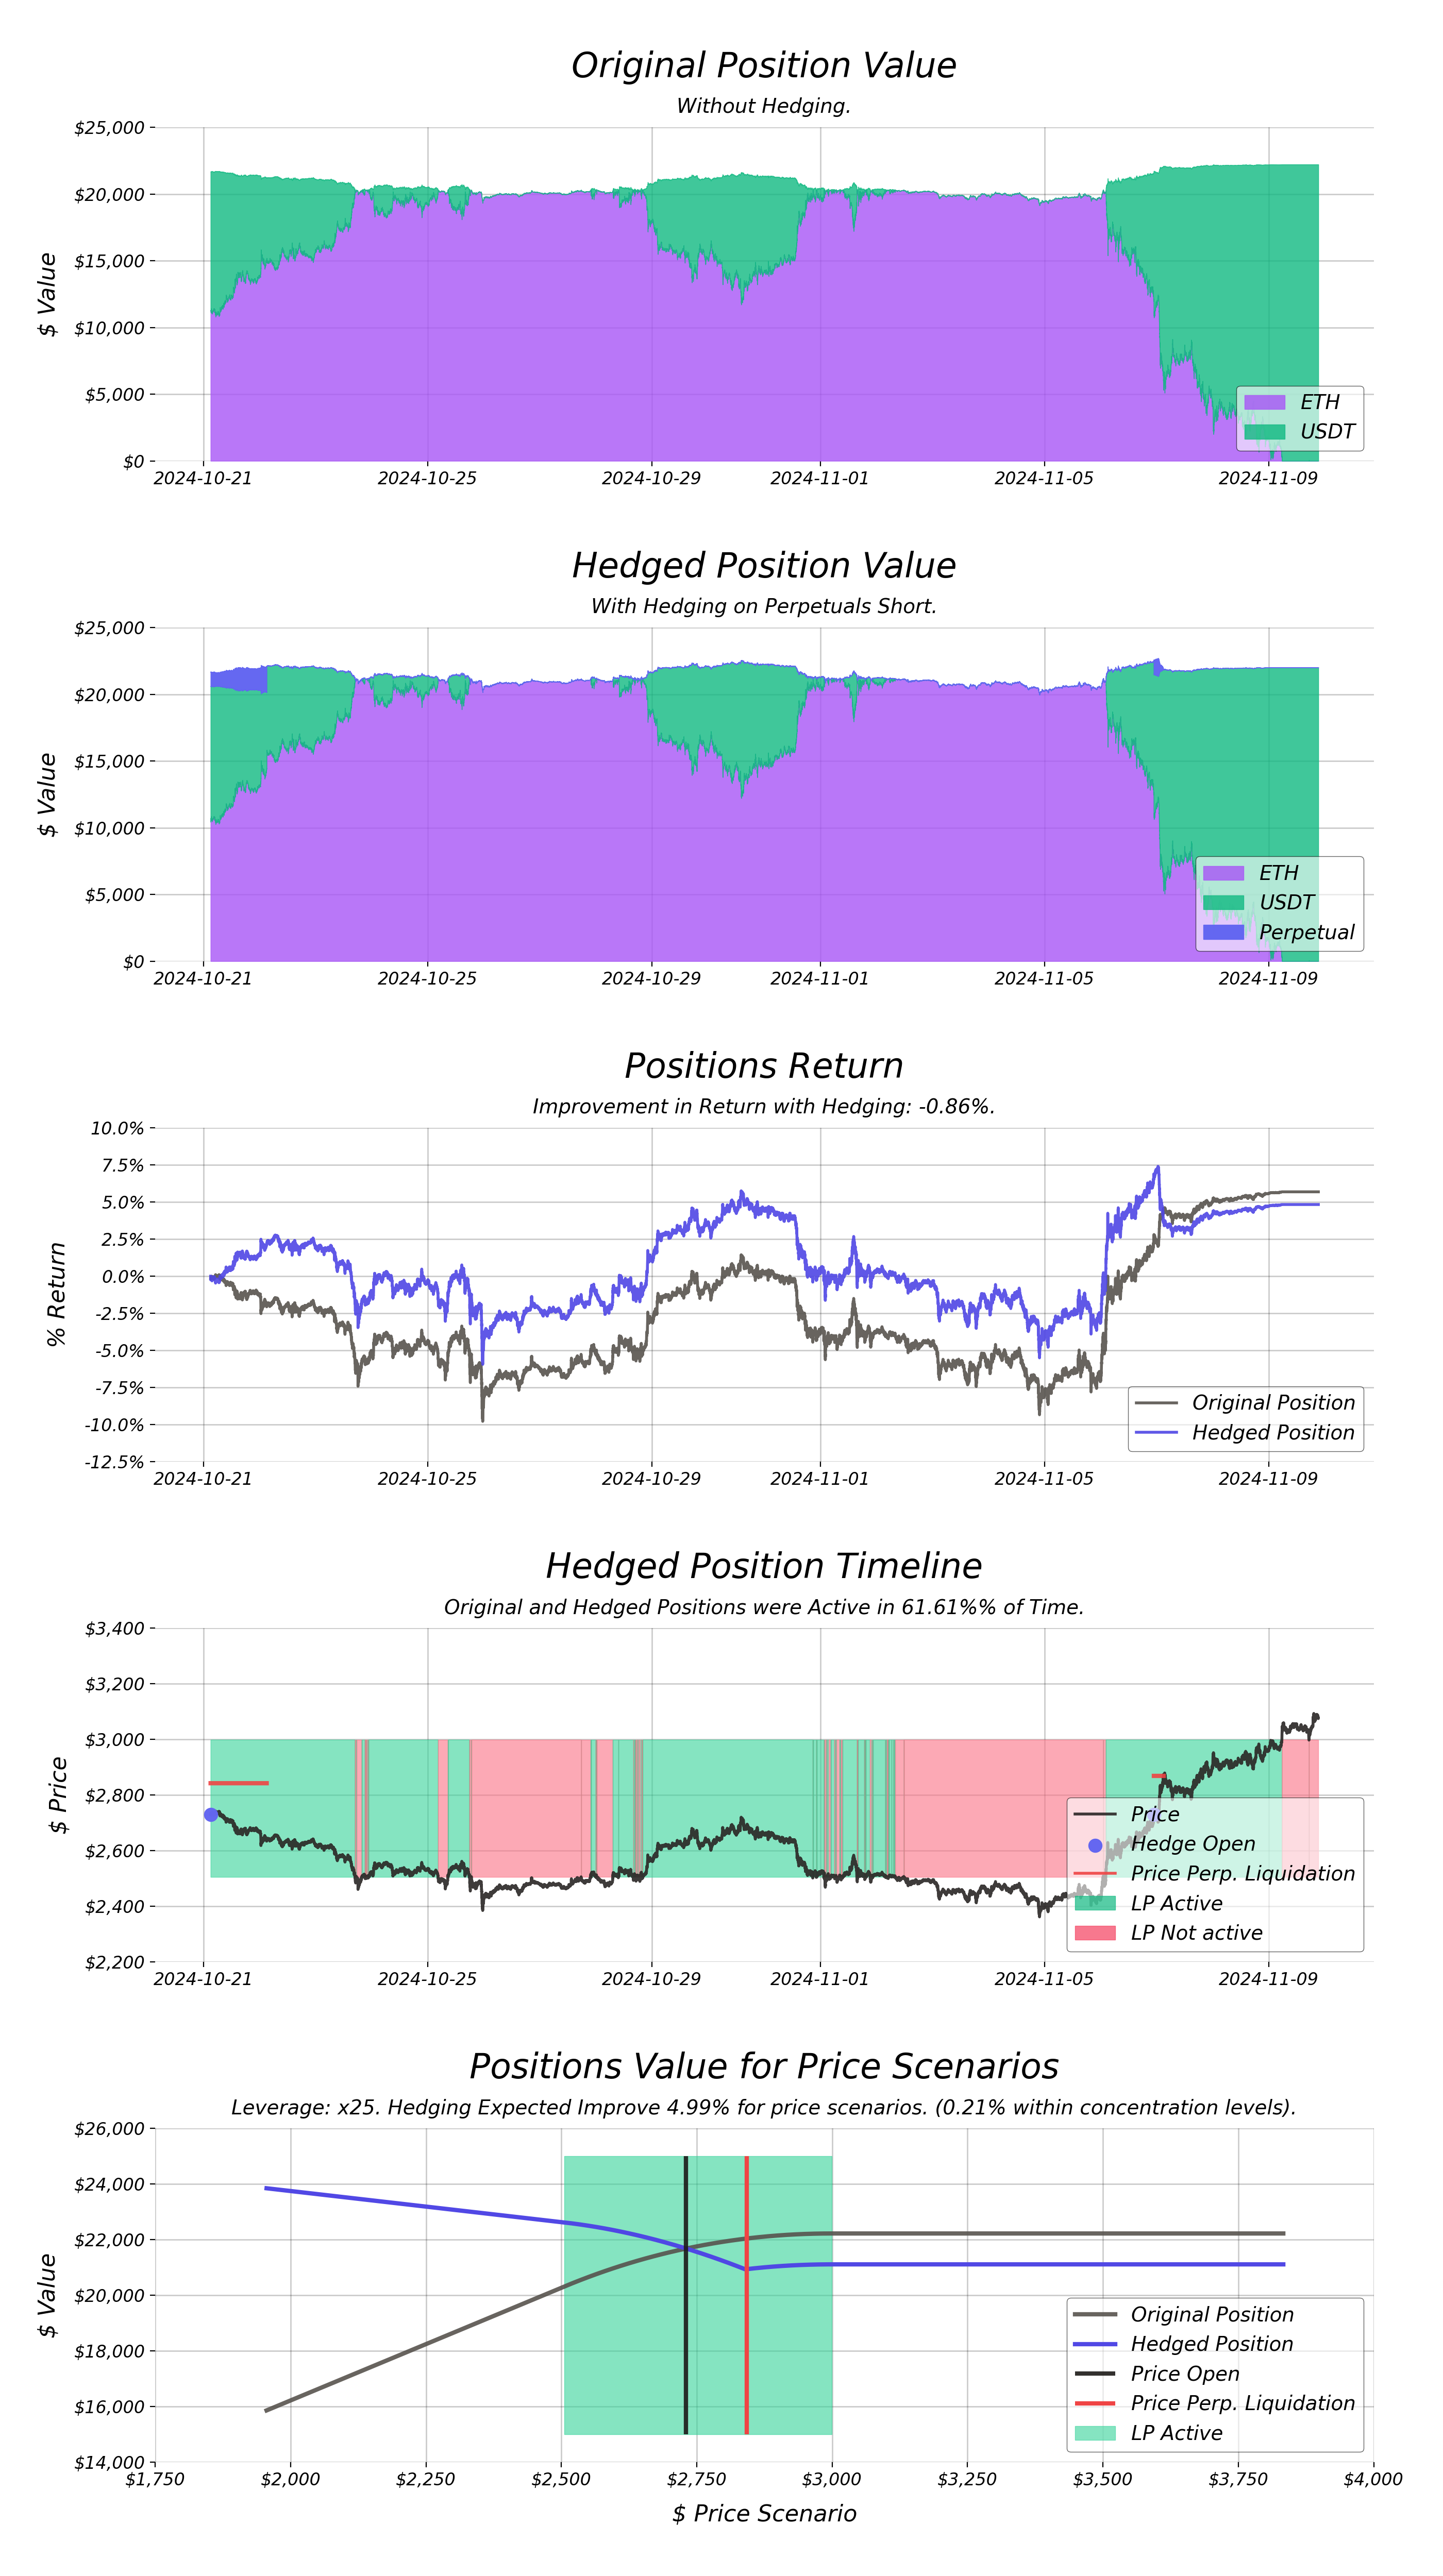
\includegraphics[width=0.7\textwidth]{images/Position Hedge 840439_0x4942e2b839fc479c27c496b7758bab94ceb6b684.png}
	\caption{illustrating the hedged V4 position timeline.}
	\label{fig:Sample}
\end{figure}

\paragraph{Aggregated Position Hedging}
For aggregated positions, we have applied extra differentiation based on market status predicted by Xtreamly AI.

\begin{table}[htb]
	\centering
	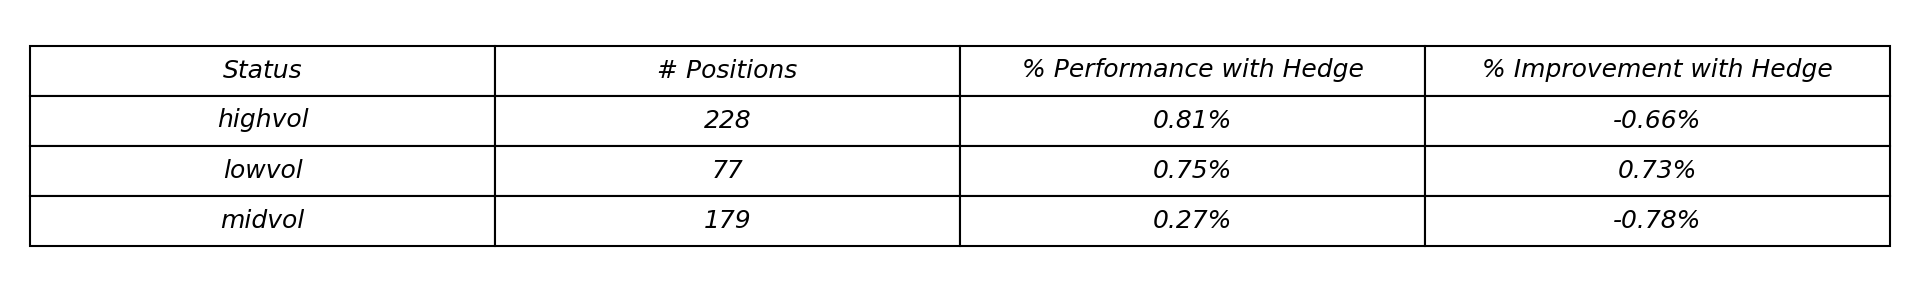
\includegraphics[width=0.99\textwidth]{images/Table Improvement.png}
	\caption{illustrating the aggregated improvement for hedged V4 position depending on market status at position open.}
	\label{fig:Agr}
\end{table}

\begin{figure}[htb]
	\centering
	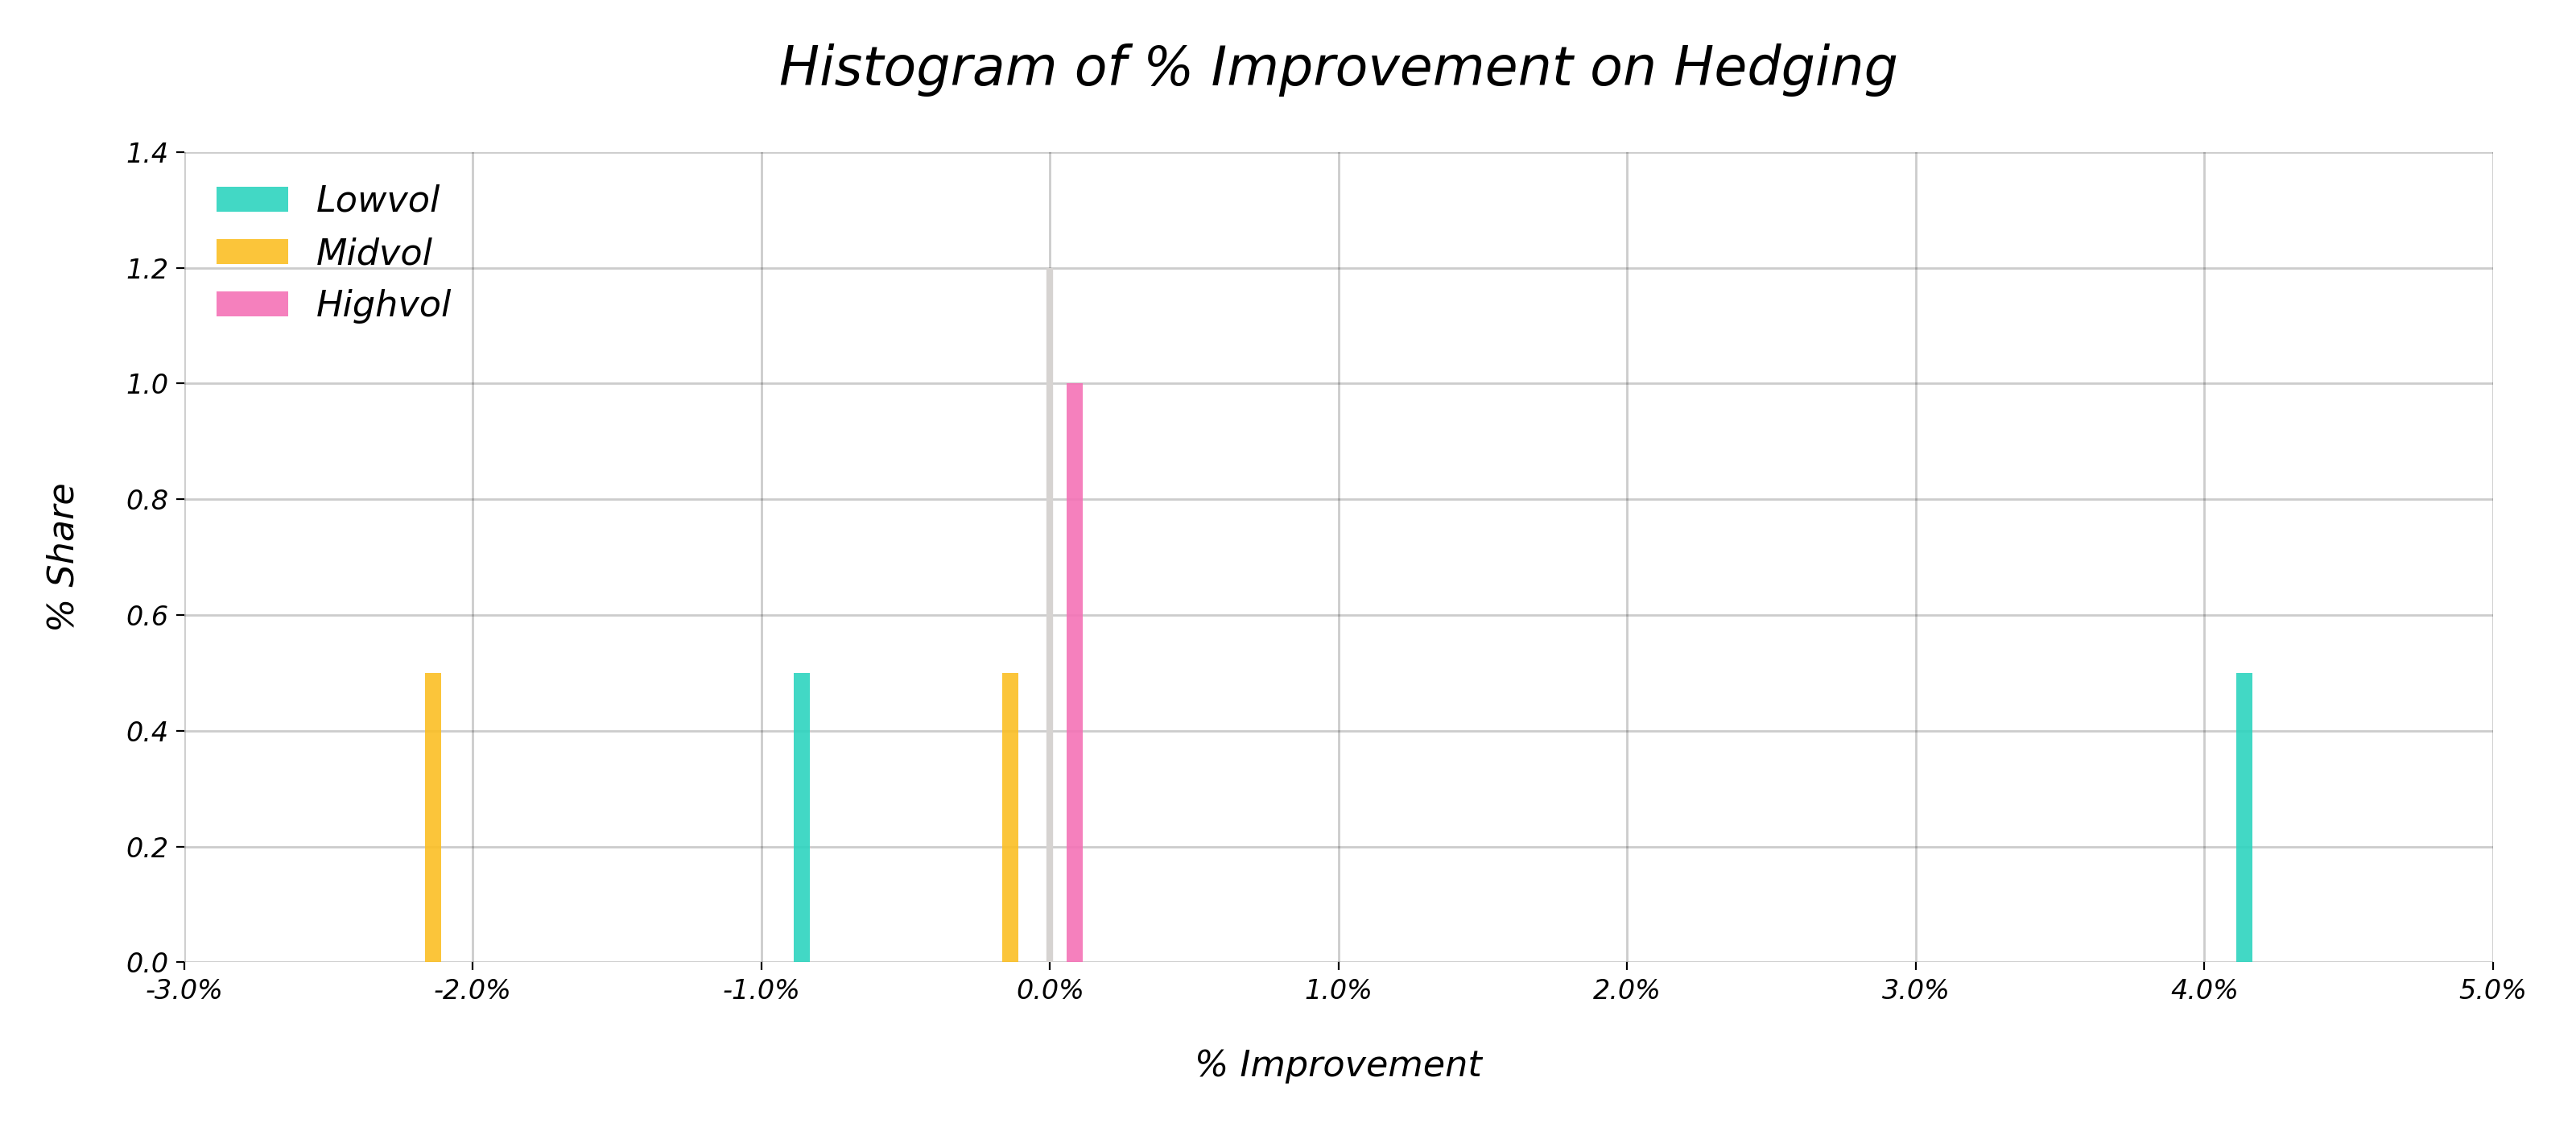
\includegraphics[width=0.8\textwidth]{images/Histogram Improvement.png}
	\caption{illustrating the improvement distribution depending on market status at position open.}
	\label{fig:HistImprov}
\end{figure}

We observe clear added value for positions opened during low volatility periods. This is partly due to the reduced perpetual liquidations as well as the skewness of the payoff function, favoring perpetuals as an implementation of a market-neutral position whenever the market regime is in low volatility.

\medskip

Intrestingly, hedging on perpetuals were positive on averge for avery market status. This positive returns, however did not payoff the collateral cost take from original LP position.

\newpage

\section{Further Work}
\label{sec:futurework}

\subsection{Further and Deeper Analysis}
Expand analysis to other pools and tokens, seeking data signals for opening perpetual hedging.

\subsection{Intelligent Hedging Momentum}
Use Xtreamly AI volatility predictions to more intelligently define opening and closing of perpetuals.

\subsection{Reinvesting Closed Perpetual into ne LP position}
Reuse PnL and collateral from closed perpetual exposure to create new LP positions, so the liquidity can be reapplied back to Uniswap and user can collect more fees.

\subsection{Automated Rebalancing and Hedging Investment Vechicle}
Develop automated rules for managing hedging exposure and rebalancing LP positions.

\subsection{New Hedging Intruments}
Explore Panoptic platform for DeFi options trading to secure hedging during high volatility periods.

\newpage

\section{Reference}
\label{sec:ref}
To fill in.
\begin{itemize}
	\item \textbf{Uniswap Documentation}
	\item \textbf{GMX Documentation}
	\item \textbf{Other}
\end{itemize}

\end{document}